% !TEX root = ../thesis.tex

\chapter{Hintergrund}

\paragraph{Ausblick:}
Zum besseren Verständnis der weiteren Verlaufs dieser Arbeit, dient dieses Kapitel zur Einführung in die zugrundeliegenden Themen. Dazu wird zunächst die featurebasierte Softwareentwicklung erläutert, ehe dann der Themenbereich des Machine Learnings vorgestellt wird. Dazu werden die Klassifikation und die Fehlervorhersage mittels Machine Learning erläutert. Unterstützt werden die Abschnitte von Grafiken zum besseren Verständnis der Zusammenhänge.
\\
\hrule

\section{Featurebasierte Softwareentwicklung}

\section{Machine-Learning-Klassifikation}

\textbf{ÜBERARBEITEN!}

Die Machine-Learning-Klassifikation unterliegt dem Teilgebiet des \emph{überwachten Machine Learnings} (englisch: supervised Machine Learning). Die nachfolgende \autoref{fig:ml} präsentiert den allgemeinen Prozess des überwachten Machine Learnings auf vereinfachter Weise anhand eines Beispiels. Anhand dieser werden die wichtigsten Informationen zum genannten Themengebiet erläutert. 

\begin{figure}[H]
    \centering
    \captionsetup{justification=centering,margin=2cm}
    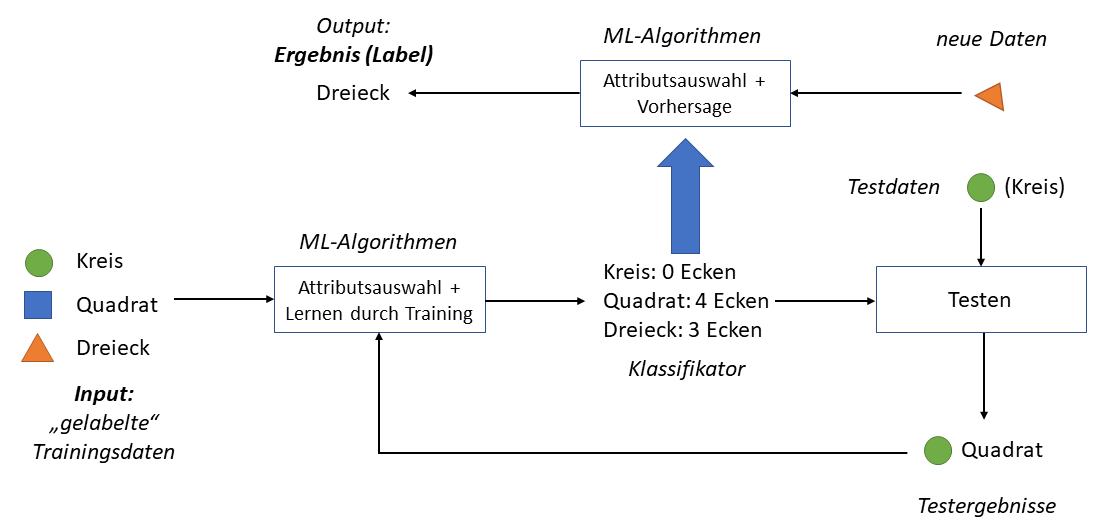
\includegraphics[width=\textwidth]{images/ML}
    \caption{Allgemeiner Prozess des überwachten Machine Learnings dargestellt anhand eines Beispiels (vereinfacht)}\label{fig:ml}
\end{figure}

Das in der Abbildung gezeigte Beispiel zeigt den Prozess der Entwicklung und Erlernung eines Klassifikators zur Erkennung von geometrischen Formen.
Der Prozess beginnt mit der Erstellung eines Datensets, welches als Input für die Erlernung des Klassifikators dient.

\textbf{ÜBERARBEITEN!}

\begin{figure}[H]
    \centering
    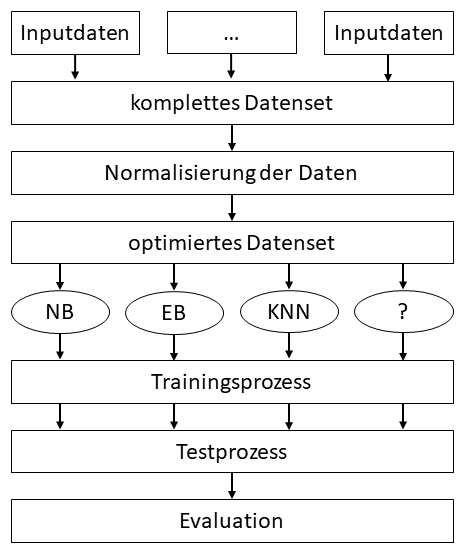
\includegraphics[width=0.5\textwidth]{images/Prozess}
    \caption{Angewendeter Prozess zur Durchführung der Klassfikation nach \cite{Ceylan2006}}\label{fig:process}
\end{figure}

\section{Fehlervorhersage mittels Machine Learning}

Der Hintergrund zur Fehlervorhersage mittels Machine Learning wird anhand eines Beispiels aus der Literatur erläutert. Es stammt aus einer wissenschaftlichen Arbeit von Queiroz et al. \cite{Queiroz2016} und widmet sich der Fehlervorsage von Features. Bei dieser ersten Fallstudie handelt es sich um die bisher einzige Arbeit mit Bezug zu Software-Features und stellt somit für diese Masterarbeit eine bedeutende literarische Grundlage dar. Der Ablauf des von Queiroz et al. angewandten Prozesses zur Erstellung eines featurebasierten Datensets und dessen Anwendung zur Erlernung von Klassifikatoren orientiert sich am zuvor vorgestellten allgemeinen Prozess des überwachten Machine Learnings.

Die Erläuterung des Beispiels erfolgt anhand von drei Abbildungen, welche den in der Arbeit von Queiroz et al. vorgestellten Prozess in drei Teilen visualisieren. 

\begin{figure}[H]
    \centering
    \captionsetup{justification=centering}
    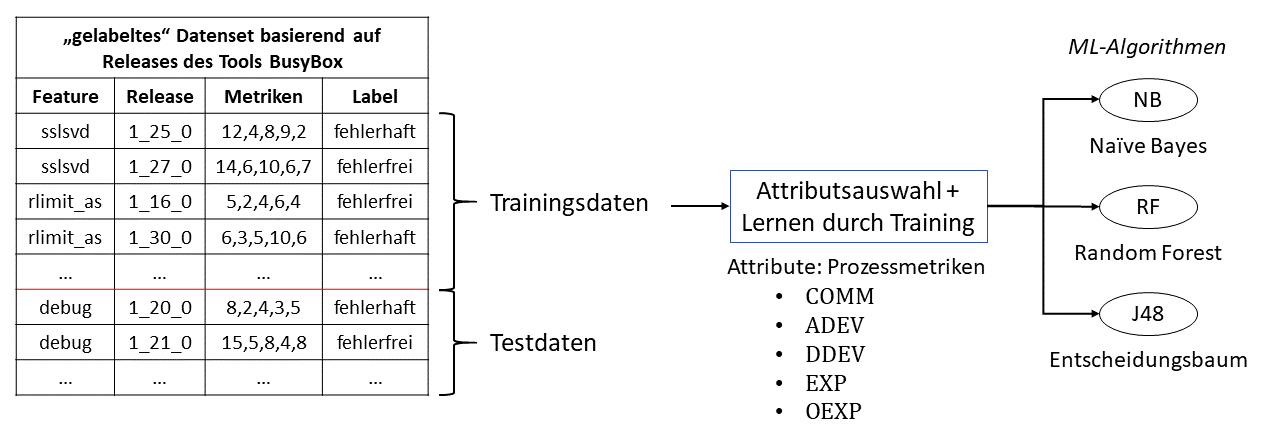
\includegraphics[width=\textwidth]{images/ML1}
    \caption{Teil 1: Featurebasierter Prozess des überwachten Machine Learnings nach \cite{Queiroz2016}}\label{fig:ml1}
\end{figure}

Die Datenbasis des Datensets bilden Commits des UNIX-Toolkits BusyBox\footnote{\url{https://busybox.net/}}, dessen Quellcode frei verfügbar in einem Git-Repository\footnote{\url{https://git.busybox.net/busybox/}} eingesehen und von dort geklont werden kann. Diese Commits wurden wiederum ihren entsprechenden Releases zugeordnet, welche auf der vergebenen Tag-Struktur des Repositories beruhen. Ferner wurden aus den Diffs der Commits die dort bearbeiteten Features extrahiert und anschließend zusammen mit den Release-Informationen in einer MySQL-Datenbank gespeichert. Zusätzlich enthält jeder Datenbankeintrag aggregierte Werte von fünf auf das Feature und den Release bezogenen Prozessmetriken (Erläuterung folgt) sowie das binäre Label, ob ein Feature in einem Release fehlerhaft oder fehlerfrei war. Ein Feature gilt in einem Release als fehlerhaft, sofern in einem Commit des darauffolgenden Releases ein fehlerbehebender Commit bezüglich des Features festgestellt werden konnte. Dies geschieht über die Analyse der Commit-Nachrichten. Sofern eine Commit-Nachricht die Begriffe \glqq bug\grqq{} (Fehler), \glqq error\grqq{} (schwerwiegender Fehler), \glqq fail\grqq{} (fehlschlagen) oder \glqq fix\grqq{} (beheben) enthält, werten die Autoren des Papers den Commit als fehlerbehebend. Wie im Rahmen des überwachten Machine Learning üblich, wird das Datenset in Trainings- und Testdaten in einem Verhältnis von 75:25 geteilt. 

\textbf{ALTERNATIVE WEGE (BUGTRACKING, SZZ), SIEHE VERGLEICHSPAPER}

Die Trainingsdaten werden dann den Klassifikatoren zur Erlernung zur Verfügung gestellt. Als Attribute dienen die fünf bereits erwähnten Prozessmetriken mit spezifischer Betrachtung von Software-Features. Die nachfolgende Tabelle gibt einen Überblick über die Beschreibungen dieser.

\begin{table}
\centering
\caption{Übersicht der von \cite{Queiroz2016} verwendeten Prozessmetriken}
\label{tab:metrics}
\begin{tabular}{c|l}
\multicolumn{1}{c|}{\textbf{Metrik} } & \textbf{Beschreibung}  \\ 
\hline
COMM & \begin{tabular}[c]{@{}l@{}}Anzahl der Commits, die in einem Release dem betreffenden \\ Feature gewidmet sind.\end{tabular} \\
ADEV & \begin{tabular}[c]{@{}l@{}}Anzahl der Entwickler, die das betreffende Feature\\in einem Release bearbeitet haben.\end{tabular} \\
DDEV & \begin{tabular}[c]{@{}l@{}}kummulierte Anzahl der Entwickler, die das betreffende Feature\\in einem Release bearbeitet haben.\end{tabular} \\
EXP & \begin{tabular}[c]{@{}l@{}}Geometrisches Mittel der \glqq Erfahrung\grqq{} aller Entwickler, die am \\ betreffenden Feature in einem Release gearbeitet haben.\end{tabular} \\
OEXP & \begin{tabular}[c]{@{}l@{}}\glqq Erfahrung\grqq{} des Entwicklers, der am meisten zum betreffenden \\ Feature in einem Release beigetragen hat.\end{tabular} \\ 
\hline
\multicolumn{2}{c}{\begin{tabular}[c]{@{}c@{}}Erfahrung ist definiert als Summe der geänderten, gelöschten\\oder hinzugefügten Zeilen im zugehörigen Release.\end{tabular}} \\
\hline
\end{tabular}
\end{table}

\begin{figure}[H]
    \centering
    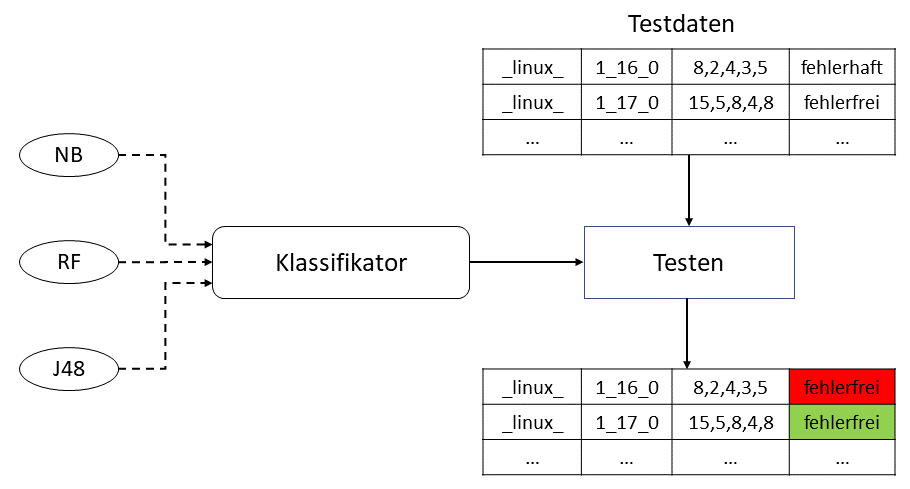
\includegraphics[width=\textwidth]{images/ML2}
    \caption{Teil 2: Featurebasierter Prozess des überwachten Machine Learnings nach \cite{Queiroz2016}}\label{fig:ml2}
\end{figure}

\begin{figure}[H]
    \centering
    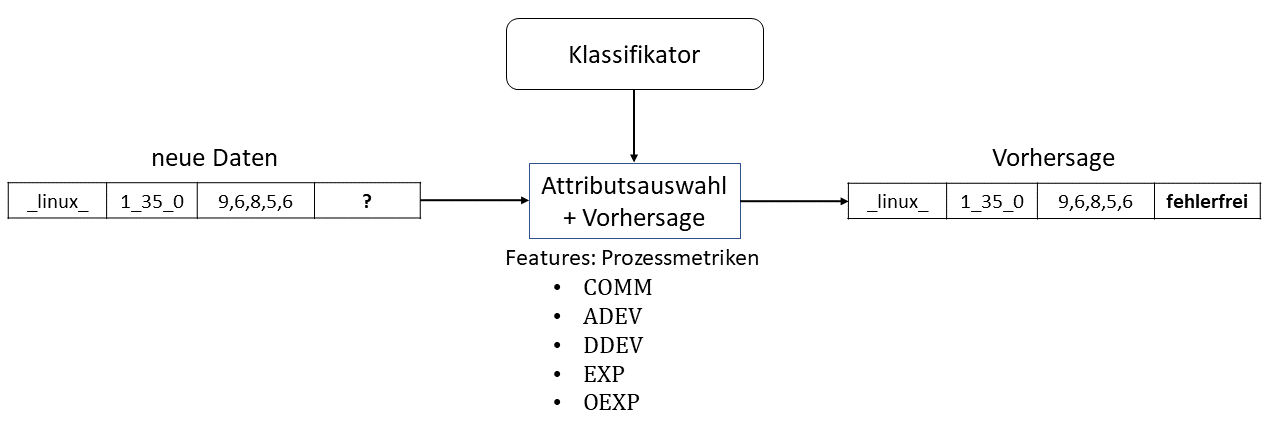
\includegraphics[width=\textwidth]{images/ML3}
    \caption{Teil 3: Featurebasierter Prozess des überwachten Machine Learnings nach \cite{Queiroz2016}}\label{fig:ml3}
\end{figure}

\cleardoublepage
